\documentclass[14pt,a4paper]{scrartcl}
\usepackage{cmap}
\usepackage[utf8]{inputenc}
\usepackage[T1,T2A]{fontenc}
\usepackage[english,russian]{babel}
\usepackage{relsize}
\usepackage{graphicx}
\usepackage{subfigure}
\usepackage{mathtools}
\usepackage{amssymb}
\usepackage{float}
\usepackage{sidecap}
\usepackage{wrapfig}
\usepackage{caption}
\usepackage[table,xcdraw]{xcolor}
\usepackage{listings}
\usepackage{amsmath,cryptocode}
\usepackage{listings}
\usepackage{booktabs}
\usepackage{multirow}  
\usepackage{multicol}
\usepackage{bigstrut}
\usepackage{lscape}
\usepackage{rotating}
\usepackage{adjustbox}
\usepackage{minted}
\usepackage{breqn}
\usepackage{physics}


\newcommand\scalemath[2]{\scalebox{#1}{\mbox{\ensuremath{\displaystyle #2}}}}


\begin{document}
	\begin{titlepage}
	\begin{center}
		\large
		МИНИСТЕРСТВО ОБРАЗОВАНИЯ И НАУКИ\\ РОССИЙСКОЙ ФЕДЕРАЦИИ
		
		\vspace{0.5cm}
		
		МГТУ им Н.Э.Баумана
		\vspace{0.25cm}
		
		Факультет ФН
		
		Кафедра вычислительной математики и математической физики
		\vfill
		
		
		Соколов Арсений Андреевич\\
		\vfill
		
		
		{\LARGE Лабораторная работа №6 по численным методам\\[2mm]
		}
		\bigskip
		
		3 курс, группа ФН11-53Б\\
		Вариант 6
	\end{center}
	\vfill
	
	\newlength{\ML}
	\settowidth{\ML}{«\underline{\hspace{0.7cm}}» \underline{\hspace{2cm}}}
	\hfill\begin{minipage}{0.4\textwidth}
		Преподаватель\\
		\underline{\hspace{3cm}} В.\,А.~Кутыркин\\
		«\underline{\hspace{0.7cm}}» \underline{\hspace{1.71cm}} 2019 г.
	\end{minipage}%
	\bigskip
	
	
	\vfill
	
	\begin{center}
		Москва, 2019 г.
	\end{center}
\end{titlepage}

\section*{Задание 1}
\textbf{Задание.}\\
На отрезке $[0;1]$ задана равномерная сетка $A = \langle \tau_0, \tau_1, \ldots, \tau_k\rangle$, где $k=40$, с шагом $h = \frac{b-a}{k} = 0.025 = stp(A)$ и определена функция $$f(\tau)=2 \sin (\pi \tau) \sqrt{55-n+N \tau \sqrt{25-N}},$$ где $N$ -- номер студента в журнале, $n$ -- номер группы. Для $A$-сеточной функции $\prescript{>}{}{y} = \hat{A}(f) = [y_0,y_1,\ldots,y_k\rangle \in \prescript{>}{}{R^{|A|}(A)}$, где $y_i=f(\tau_i)$ для $i=0,1,\ldots,k$, решить задачу $A-$интерполяции сеточной функции $\prescript{>}{}{y}$ с помощью сплайна $spl_2(A;\prescript{>}{}{y})$ 2-ой степени дефекта 1. Затем сравнить в узлах интерполяции равномерной сетки $A = \langle \tau_0, \tau_1, \ldots, \tau_k\rangle $ отрезка $[0;1]$ значения производный от функции $f(\tau)$ и сплайна $spl_2(A;\prescript{>}{}{y})$, т.е. значения функций $\dv{f}{\tau}$ и $\dv{spl_2(A;\prescript{>}{}{y})}{\tau}$


\textbf{Исходные данные.}\\
$N = 6, n = 53$

\begin{equation*}
f(\tau) = 2 \sin (\pi \tau) \sqrt{55-n+N \tau \sqrt{25-N}} =2\,\sin \left( \pi\,\tau \right) \sqrt {2+6\,\tau\,\sqrt {19}}
\end{equation*}

\textbf{Решение.}\\
На отрезке $[0;1]$ задана равномерная сетка $A = \langle \tau_0, \tau_1, \ldots, \tau_k\rangle$, где $k=40$, с шагом $h = \frac{b-a}{k} = 0.025 = stp(A)$. Получаем узлы:

\begin{figure}[h]
	\center{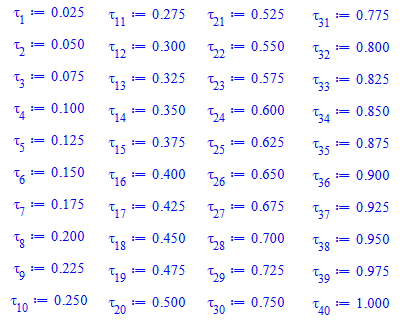
\includegraphics[width=0.75\linewidth]{../img/uzli.png}}
\end{figure}


Для $A$-сеточной функции $\prescript{>}{}{y} = \hat{A}(f) = [y_0,y_1,\ldots,y_k\rangle \in \prescript{>}{}{R^{|A|}(A)}$, где $y_i=f(\tau_i)$ для $i=0,1,\ldots,k$, получаем:

\begin{figure}[h]
	\center{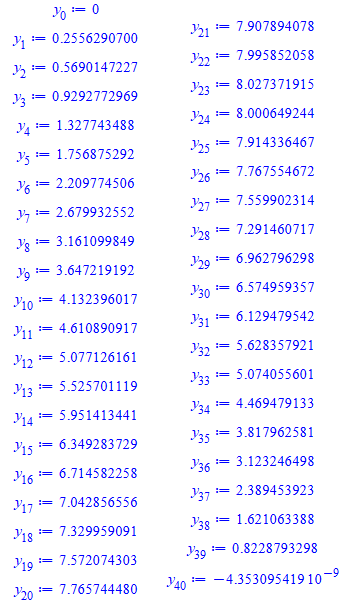
\includegraphics[width=0.66\linewidth]{../img/a_set.png}}
\end{figure}


Если сетка $A = \langle a=\tau_0, \tau_1, \ldots, \tau_k=b\rangle$ является равномерной и ее шаг $h = \frac{b-a}{k} = 0.025 = stp(A)$, то для $i=1,2,\ldots,k$ на отрезке $[\tau_{i-1};\tau_i]$ находятся значения коэффициентов полинома $p_i(\tau) = a_i + b_i(\tau-\tau_{i-1}) + c_i(tau-tau_{i-1})^2$:
\begin{equation*}
a_1 = y_0, \quad b_1 = \frac{y_1-y_0}{h}, \quad c_1 = 0
\end{equation*}
\begin{equation*}
a_i = y_{i-1}, \quad b_i = b_{i-1} + 2c_{i-1}h, \quad c_i = \frac{y_i - y_{i-1} - (b_{i-1} + 2c_{i-1}h)h}{h^2}, \quad i=2,3,\ldots,k
\end{equation*}

Получаем:
\begin{figure}[h]
	\center{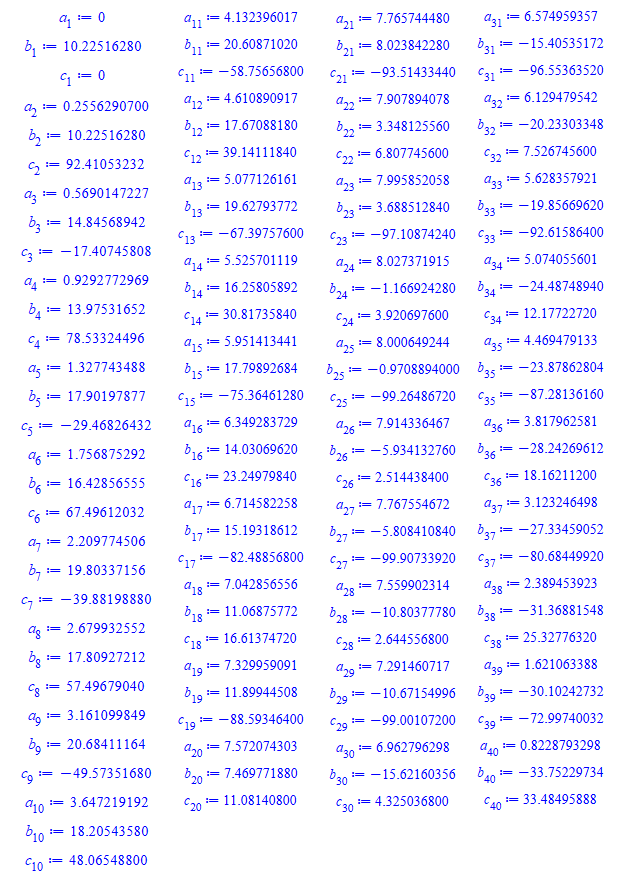
\includegraphics[width=0.75\linewidth]{../img/cifri.png}}
\end{figure}

Построим совмещенные графики функции $f(\tau)$ и $spl_2(A;\prescript{>}{}{y})$ интерполяционного сплайна 2-ой степени дефекта 1.
\pagebreak

\begin{figure}[t]
	\center{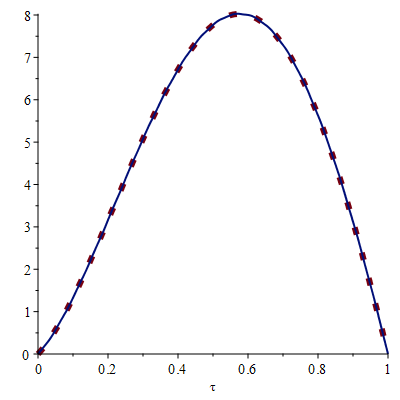
\includegraphics[width=0.95\linewidth]{../img/graa1.png}}
\end{figure}
Как видим, полином ложится на нашу функцию.

\clearpage
В узлах интерполяции равномерной сетки $A = \langle \tau_0, \tau_1, \ldots, \tau_k\rangle$ отрезка $[0;1]$ найдём значения производный от функции $f(\tau)$ и сплайна $spl_2(A;\prescript{>}{}{y})$, т.е. значения функций $\dv{f}{\tau}$ и $\dv{spl_2(A;\prescript{>}{}{y})}{\tau}$:

\begin{equation*}
	2\,\pi\,\cos \left( \pi\,\tau \right) \sqrt {2+6\,\tau\,\sqrt {19}}+6
	\,{\frac {\sin \left( \pi\,\tau \right) \sqrt {19}}{\sqrt {2+6\,\tau\,
				\sqrt {19}}}}
\end{equation*}


Построим совмещенные графики функций $\dv{f}{\tau}$ (кривая) и $\dv{spl_2(A;\prescript{>}{}{y})}{\tau}$ (точки, соединенные отрезками прямой):

\begin{figure}[h]
	\center{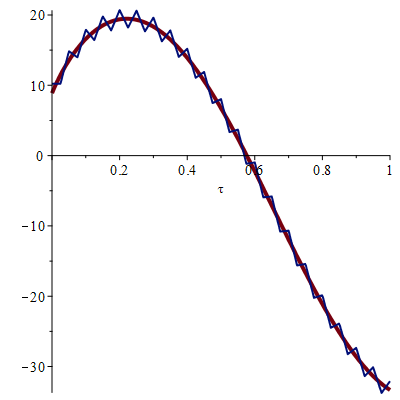
\includegraphics[width=0.75\linewidth]{../img/graa2.png}}
\end{figure}

Видим, что графики хорошо наложились

\textbf{Выводы.}
В результате работы было графически проиллюстрировано, что интерполяционный сплайн $spl_2(A;\prescript{>}{}{y})$ 2-ой степени дефекта 1 для $A-$ сеточной функции $\prescript{>}{}{y} = \hat{A}(f) = [y_0,y_1,\ldots,y_k\rangle \in \prescript{>}{}{R^{|A|}(A)}$, где $y_i=f(\tau_i)$ для $i=0,1,\ldots,k$ хорошо накладывается на функцию $f(\tau)$. А в узлах равномерной сетки $A = \langle \tau_0, \tau_1, \ldots, \tau_k\rangle$ отрезка $[0;1]$ значения производных функции $f(\tau)$ и сплайна $spl_2(A;\prescript{>}{}{y})$, то есть значения функций $\dv{f}{\tau}$ и $\dv{spl_2(A;\prescript{>}{}{y})}{\tau}$ близки друг к другу.

\end{document}